
    \documentclass[tikz,convert={outfile=\jobname.png}]{standalone}
    \usetikzlibrary{mindmap,trees,backgrounds}
    \usepackage{fontspec}
    \usepackage{lmodern}
    \defaultfontfeatures{Ligatures=TeX,Scale=3}
    \setmainfont{M+ 1mn}
    
    
    \definecolor{metallic}{RGB}{0, 121, 140}
    \definecolor{tc}{RGB}{209, 73, 91}
    \definecolor{yellow}{RGB}{237, 174, 73}
    \definecolor{shamrock}{RGB}{102, 161, 130}
    \definecolor{nvy}{RGB}{46, 64, 87}
    \definecolor{vio}{RGB}{156, 100, 123}
    \definecolor{orng}{RGB}{239, 138, 23}
    \definecolor{white}{RGB}{255.0, 255.0, 255.0}
    \definecolor{dimgray}{RGB}{104.55, 104.55, 104.55}
    
    \begin{document}
    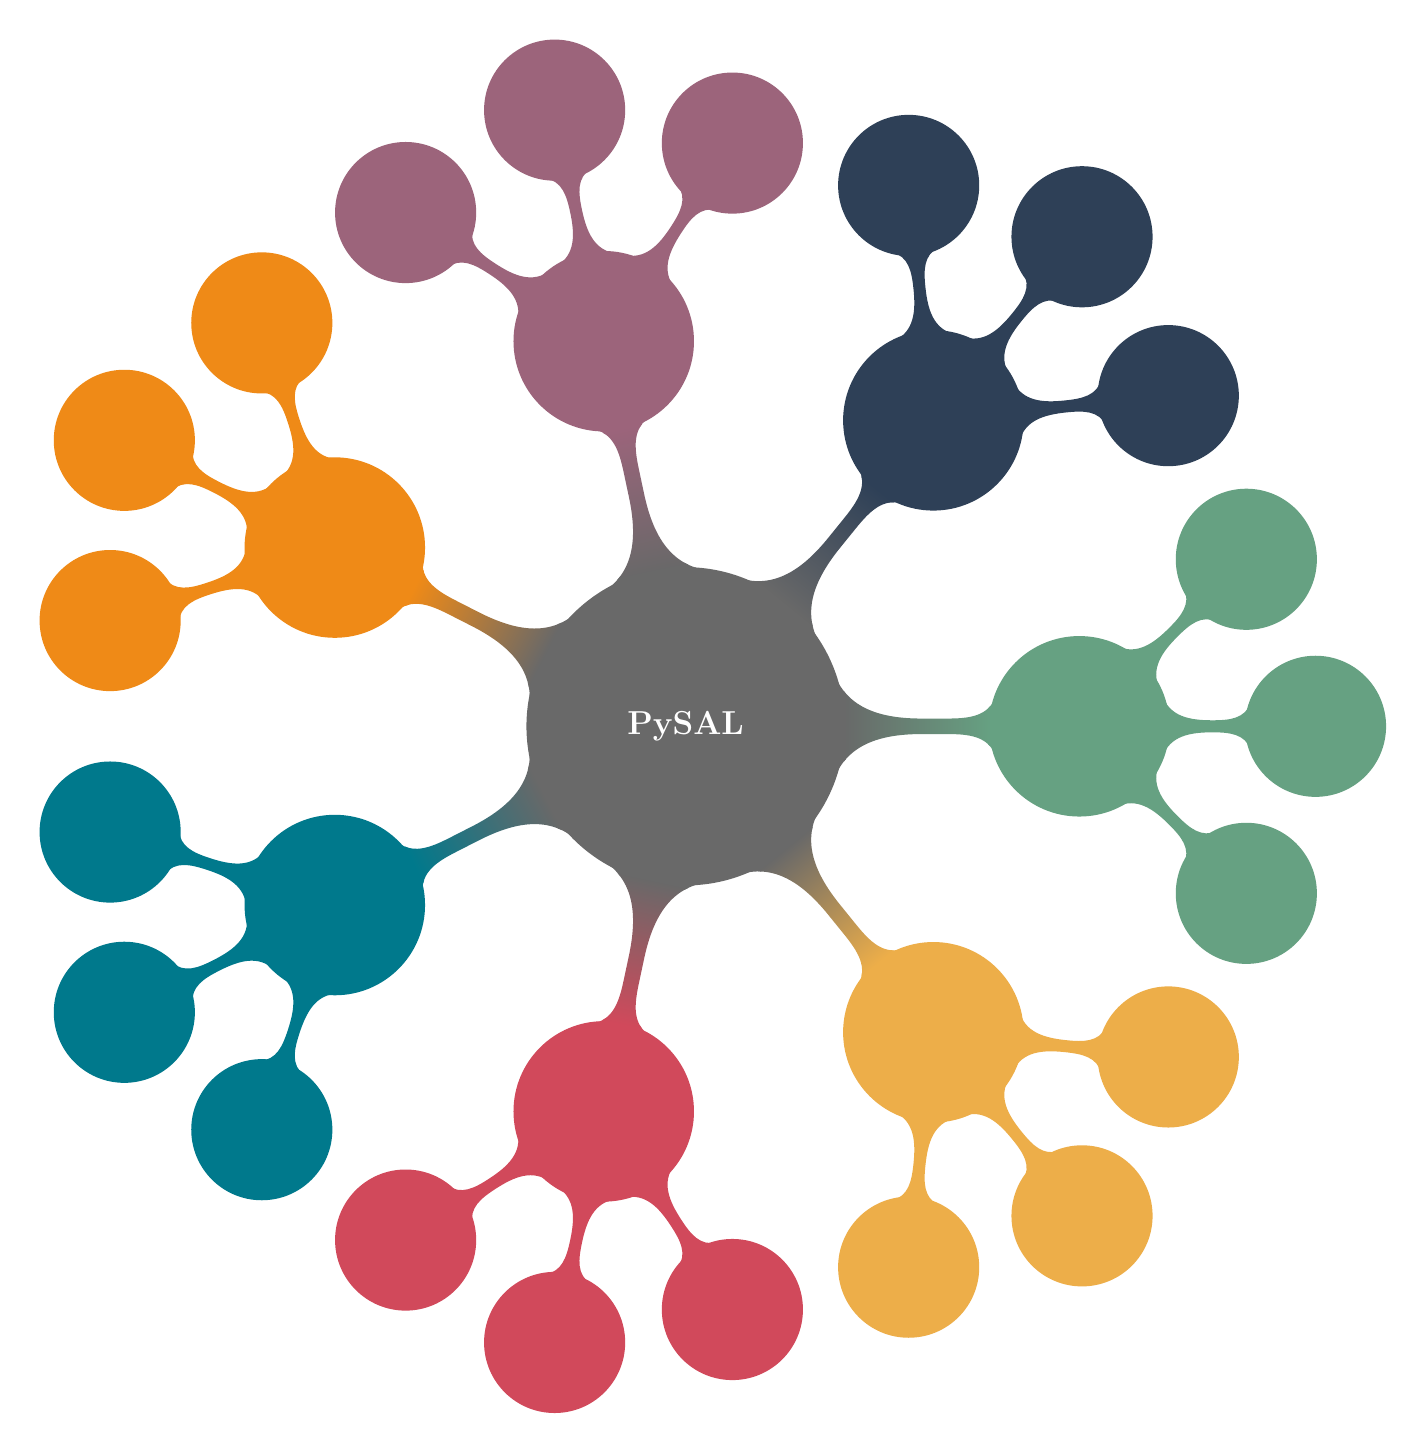
\begin{tikzpicture}[
        background rectangle/.style={fill=white},
        show background rectangle,
        mindmap,
        grow cyclic,
        every node/.style=concept,
        concept color=dimgray,
        text=white,
        level 1/.append style={
            level distance=5cm,
            sibling angle=51,
            font=\Huge
        },
        level 2/.append style={
            level distance=3cm,
            sibling angle=45
        }
    ]
    
        \node[concept color=dimgray]{\large\bfseries{PySAL}}
        child [concept color=metallic]{ node {}
            child { node { }}
            child { node { }}
            child { node { }}
         }
        child [concept color=tc]{ node {}
            child { node { }}
            child { node { }}
            child { node { }}
         }
        child [concept color=yellow]{ node {}
            child { node { }}
            child { node { }}
            child { node { }}
         }
        child [concept color=shamrock]{ node {}
            child { node { }}
            child { node { }}
            child { node { }}
         }
        child [concept color=nvy]{ node {}
            child { node { }}
            child { node { }}
            child { node { }}
         }
        child [concept color=vio]{ node {}
            child { node { }}
            child { node { }}
            child { node { }}
         }
        child [concept color=orng]{ node {}
            child { node { }}
            child { node { }}
            child { node { }}
         }
                ;
    
    \end{tikzpicture}
    \end{document}